\begin{frame}{Cross-Validation}{Leave-one-out cross-validation}

\begin{itemize}
    \item Split the set of observations into two parts: \pause 
    \begin{enumerate}
        \item A single observation $(x_1 , y_1 )$, used as the validation set. \pause
        \item The remaining observations $\{(x_2 , y_2 ), \cdots , (x_n, y_n )\}$, used as the training set. \pause
    \end{enumerate}
    
    \item Fit the model on the $n - 1$ training observations. \pause 
    
    \item Make a prediction $\hat{y}_1$ for the excluded observation, using its value $x_1$. \pause

    \item Since $(x_1 , y_1)$ was not used in the fitting process, $MSE_1 = (y_1 - \hat{y}_1 )^2$ provides an approximately \textbf{unbiased} estimate for the test error. \pause 
    
    \item However, it is a poor estimate because it is highly variable. \pause \\  
    $\rightarrow$ It is based upon a single observation $(x_1 , y_1)$. \pause

    \item Repeating this approach $n$ times produces $n$ squared errors. \pause \\
    $\rightarrow$  Select $(x_2 , y_2 )$ as the validation data, train the model on $\{(x_1 , y_1 ), (x_3 , y_3 ) \cdots , (x_n, y_n )\}$ and compute $MSE_2 = (y_2 - \hat{y}_2 )^2$. \pause
 
    \begin{equation}
        CV_{n} = \frac{1}{n} \sum_{i=1}^n MSE_i. 
    \end{equation}
    
\end{itemize}
    
\end{frame}


\begin{frame}{Cross-Validation}{Leave-one-out cross-validation}

\begin{figure}
    \centering
    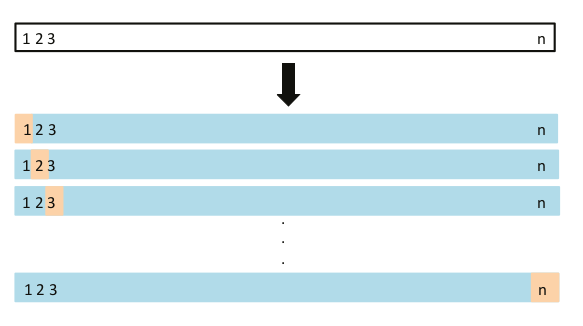
\includegraphics[height=4cm]{cross-val/l-o-o-cv.png}
\end{figure} \pause 

\begin{itemize}
    \item This approach has less bias than the validation set approach. \\ \pause  
    $\rightarrow$ Does not overestimate the test error rate as much as the validation set approach does. \pause 
    
    \item Performing LOOCV multiple times will always yield the same results. \\ \pause 
    $\rightarrow$ There is no randomness in the training/validation set splits.
\end{itemize}
    
\end{frame}


\begin{frame}{Cross-Validation}{Leave-one-out cross-validation}

\begin{block}{\textbf{Drawbacks:}}

    \begin{itemize}
        \item LOOCV has the potential to be expensive to implement, since the model has to be fit $n$ times. \pause 

        \item This can be very time consuming if $n$ is large, and if
each individual model is slow to fit.
    \end{itemize}

\end{block}

    
\end{frame}